\section{Аналитическая часть}

В данном разделе анализируется предметная область, классифицируются виды защиты от неправомерного доступа, рассматриваются базовые понятия, используемые при реализации таких методов, анализируются существующие решения, рассматривается метод хранения данных в движке MergeTree СУБД ClickHouse и модификация этого метода, предоставляющая возможность доказательства неправомерного доступа.

\subsection{Анализ предметной области}

\subsubsection{Виды защиты информации при блочном хранении данных}

Задача по обеспечению защиты от неправомерного доступа может решаться на нескольких уровнях:
\begin{enumerate}
	\item Отсутствие возможности неправомерного доступа. Самый желаемый уровень, при котором лицо не имеет возможности превышения прав при работе с информацией. Для чтения, например, может достигаться за счет шифрования данных на диске, где ключ шифрования имеется только у лиц, обладающими правами на чтение.
	\item Наличие возможности устранения последствий неправомерного доступа. Данный уровень может быть использован совместно с исключением неправомерного доступа, обеспечивая дополнительную защиту. Примерами методов защиты, обеспечивающими описанную возможность, могут послужить резервное копирование и репликация данных.
	\item Наличие возможности доказательства неправомерного доступа. Данный уровень служит для ответа на вопрос, являются ли данные консистентными. Для обеспечения такой возможности может использоваться, например, расчет контрольных сумм.
\end{enumerate}

При этом в общем случае работа с блочным хранилищем данных подразумевает 3 действия:
\begin{enumerate}
	\item [---] чтение;
    \item [---] изменение;
	\item [---] удаление блока.
\end{enumerate}

При обеспечении защиты на уровне возможности устранения последствий неправомерного доступа, восстановление данных при изменении и удалении возможно при наличии в системе избыточной информации об удаленных или измененных фрагментах. Данное условие накладывает некоторые ограничения на операции изменения и удаления. Таким образом для рассматриваемого уровня защиты можно ввести 2 дополнительные неправомерные операции:

\begin{enumerate}
	\item [---] частичное удаление блоков;
    \item [---] частичное изменение (или изменение части блоков).
\end{enumerate}

Стоит также учесть, что меры защиты применимы не ко всем операциям. Например, невозможно устранить последствия неправомерного чтения. С учетом этого и всего вышесказанного можно выделить итоговый список видов защиты информации, которые могут обеспечиваться блочным хранилищем данных:
\begin{itemize}
	\item [---] исключение неправомерного чтения;
	\item [---] исключение неправомерного изменения;
	\item [---] исключение неправомерного удаления блока;
	\item [---] возможность устраненения последствий частичного неправомерного удаления блока;
	\item [---] возможность устраненения последствий частичного неправомерного изменения;
	\item [---] доказательство неправомерного удаления блока;
	\item [---] доказательство неправомерного изменения.
\end{itemize}


\subsection{Базовые понятия}

\subsubsection{Хеш-функция}

Хеш-функции применяются:
\begin{itemize}
	\item[---] при решении задачи дедубликации;
	\item[---] при построении идентификаторов;
	\item[---] при вычислении контрольных сумм;
	\item[---] при хранении паролей.
\end{itemize}

При рассмотрении хеш-функций под алгоритмом подразумевается процесс вычисления значения хеш-функции, а под атакой на алгоритм --- решение обратной задачи: нахождение для заданного значения хеш-функции $H_1$ такого массива входных данных $A_1$, что $f(A_1) = H_1$. Хеш-функцию, которая является стойкой по определению криптографической стойкости по отношению к такой задаче, называют криптостойкой.

Криптостойкие функции также обладают следующим свойством: при наличии массива входных данных $A_1$ и значения хеш-функции для него $f(A_1)$, настолько же сложной задачей, что и нахождения обратного значения, является задача нахождения такого отличного от $A_1$ значения массива входных данных $A_2$, для которого верно $f(A_1) = f(A_2)$. Такие значения $A_1$ и $A_2$, для которых верно равенство $f(A_1) = f(A_2)$, называются коллизиями.

Схематично хеш-функция показана на рисунке \ref{fig:hashfunction}.

\begin{figure}[hbtp]
	\centering
	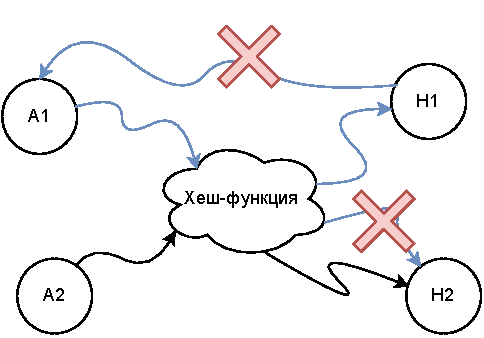
\includegraphics[scale=1]{img/hash-func.pdf}
	\caption{Хеш-функция.}
	\label{fig:hashfunction}
\end{figure}

\subsubsection{Блокчейн}

Блокчейн --- выстроенная по определенным правилам непрерывная последовательная цепь блоков --- элементов, содержащих информацию. \cite{bitcoin} В общем случае такая цепь поддерживает 2 операции:
\begin{enumerate}
    \item построение цепи (в частном случае элемент добавляется в конец и для цепи вычисляется только новое одно значение);
	\item проверка целостности всей цепи.
\end{enumerate}

При добавлении блока вычисляется значения хеша от его содержимого и хеша предыдущего блока. Вычисленное значение считается хешом добавляемого блока.

Пример блокчейна изображен на рисунке \ref{fig:blockchain}.

\begin{figure}[hbtp]
	\centering
	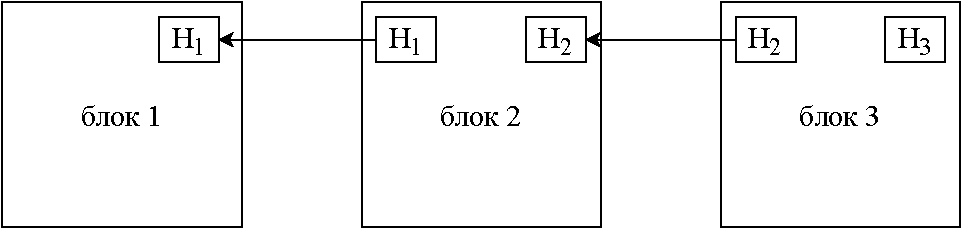
\includegraphics[width=\textwidth]{img/blockchain.pdf}
	\caption{Пример блокчейна}
	\label{fig:blockchain}
\end{figure}

При проверке целостности цепи выполняются следующие действия:
\begin{enumerate}
	\item Высчитывается хеш от содержимого первого блока и сравнивается со значением хеша, записанным при добавлении данного блока в цепь. Если значения не совпадают, то констатируется факт нарушения целостности.
	\item Для очередного блока вычисляется значение хеша от его содержимого и хеша предыдущего блока. Вычисленное значение сравнивается со значением хеша, записанным при добавлении блока. При несовпадении констатируется факт нарушения целостности.
\end{enumerate}

При изменении последнего блока достаточно пересчитать и перезаписать значения хеша только для него. Однако при изменении хеша блока, не являющегося последним, потребуется пересчитать значение хеша всех последующих блоков, что в некоторых системах может потребовать больших вычислительных затрат.

\subsubsection{Дерево и ориентированный ациклический граф Меркла}

Дерево Меркла \cite{merkle} --- двоичное дерево, в листовые вершины которого помещены хеши блоков данных, а внутренние вершины содержат хеши суммы значений в дочерних вершинах. В общем случае операция сложения --- произвольная функция от 2 аргументов \textit{f(x, y)}, которая может быть несимметричной (например, конкатенация строк). Корневой узел дерева содержит хеш от всего набора данных, то есть такое дерево является хеш-функцией.

Пример дерева Меркла можно увидеть на рисунке \ref{fig:mtree}.

\begin{figure}[hbtp]
	\centering
	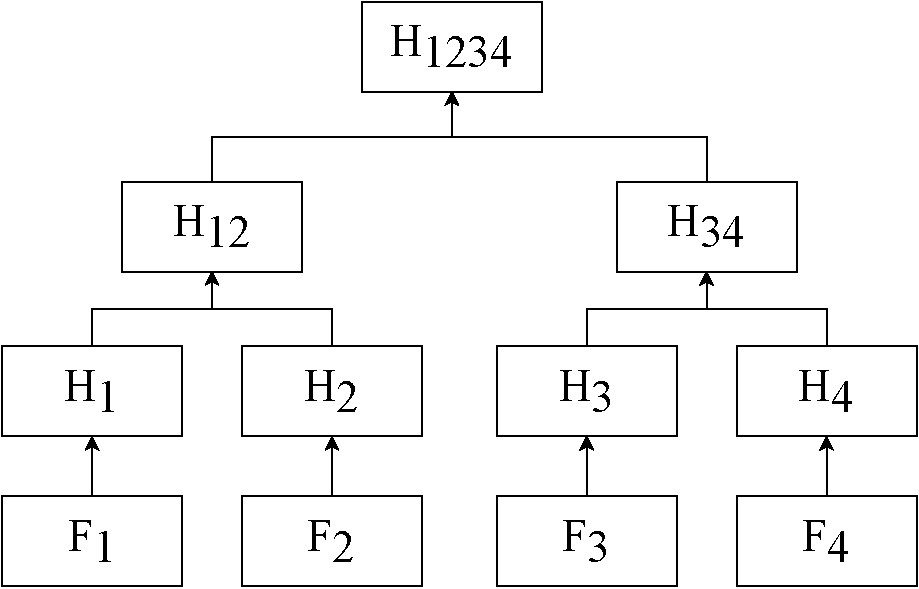
\includegraphics[width=\textwidth]{img/merkletree.pdf}
	\caption{Пример дерева Меркла}
	\label{fig:mtree}
\end{figure}

Применения дерева Меркла:
\begin{itemize}
	\item[---] Хранение транзакций в блокчейне криптовалют (например, в Bitcoin; позволяет получить значение хеша всех транзакций в блоке, а также эффективно верифицировать транзакции).
	\item[---] Для множества значений в среде с ограничением по памяти. В среде хранится только корень дерева. Для проверки принадлежности элемента множеству вместе с элементом требуется передать доказательство Меркла --- значения всех хешей, с которыми суммируется хеш проверяемого элемента на пути из листа в корень.
\end{itemize}

Ориентированный ациклический граф Меркла \cite{merkledag} --- структура данных, представляющая собой граф, строящийся по следующим правилам:
\begin{enumerate}
	\item Все вершины графа, степень полуисхода \cite{graphs} которых равна 0, представляют хеши данных.
	\item Вычисление значений остальных вершин графа делается в порядке, обратном топологической сортировке \cite{topsort}. Хешем очередной вершины будет значение хеша от суммы вершин, в которые есть дуга из рассматриваемой вершины.
\end{enumerate}

Данная структура данных используется в системе версионного контроля Git \cite{git}.

\subsection{Существующие решения}

\label{par:mainanal}

\subsubsection{PASIS}

\label{par:pasis}

PASIS \cite{pasis} --- распределенное хранилище данных, реализующее метод хранения, защищающий от ошибок, связанных с подменой данных определенными узлами системы, называемыми византийскими. Узлы хранилища хранят данные фрагментами и версионируют информацию. Клиенты читают и пишут фрагменты данных.

Данные клиента распределяются по фрамгентам на \textit{N} узлов хранилища. При чтении данных клиент обращается к \textit{m} узлам, которые являются подмножеством узлов, на которые происходила запись, и проверяет валидность полученных фрагментов. Процесс чтения может быть выполнен в несколько итераций, если в результате валидации будет выявлена ошибка. Процесс чтения считается завершенным, если получено \textit{m} верных фрагментов. Каждый отдельный фрагмент не несет в себе информации, исходные данные можно восстановить только по \textit{m} и большему числу фрагментам.

Данные восстанавливаются из фрагментов с помощью стирающих кодов \cite{erasurecode} и проверяются с помощью объединенных контрольных сумм \cite{pasis}. Объединенная контрольная сумма --- конкатенация хешей всех \textit{N} записываемых фрагментов. После восстановления данных в наличии у читателя имеются все \textit{N} фрагментов, для которых можно рассчитать значение хеша и проверить подлинность данных.

Таким образом использование данной системы позволяет защититься от неправомерного изменения или удаления данных на части узлов хранилища с возможностью восстановления данных, а также доказать неправомерное изменение данных.

\subsubsection{Криптографические файловые системы}

TCFS\cite{tcfs}, NCryptFS\cite{ncryptfs} --- примеры криптографических файловых систем. В отличие от обычных файловых систем, данные системы имеют дополнительный слой между виртуальной файловой системой и драйвером файловой системы, который шифрует данные. При такой реализации работа слоя шифрования данных будет прозрачна для пользователя, потому что пользователь работает с виртуальной файловой системой. схематично, устройство криптографической файловой системы показано на рисунке \ref{fig:cryptfs}.

\begin{figure}[hbtp]
	\centering
	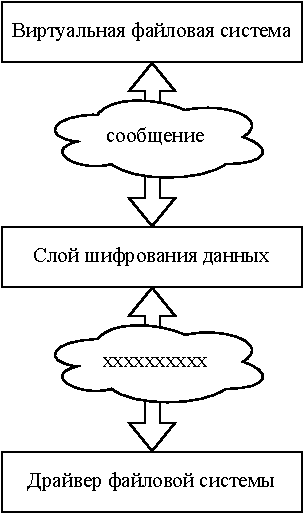
\includegraphics[scale=1]{img/cryptfs.pdf}
	\caption{Схема устройства криптографической файловой системы.}
	\label{fig:cryptfs}
\end{figure}

TCFS использует стандартные для файловых систем способы подключения в ОС \texttt{Linux}: системные вызовы \texttt{mount}, \texttt{ioctl} \cite{linux}. При работе в пределах смонтированной файловой системы все операции записи и чтения проходят через слой шифрования, поэтому данные записываются на устройство только в зашифрованном виде.

NCryptFS обладает похожим принципом работы, однако подключается с помощью собственной команды \texttt{attach}, не используя стандартные методы, и имеет возможность создания пространства имен для управления правами групп пользователей на доступ к определенным директориям, а также содержит средства авторизации.

Описанные системы решают задачу неправомерного чтения. При случайной записи данных на устройство будет нарушена их целостность, проверка целостности возлагается на приложения, использующие данные файловые системы, но так как данные хранятся в зашифрованном виде, целостность исходных данных может быть нарушена более значительно. Возможности восстановления данных нет.

\subsubsection{OceanStore}
\label{par:ocean}

OceanStore \cite{ocean} --- безопасная распределенная read-only файловая система.

Данное хранилище хранит данные в одноранговой сети, где узлы соединены между собой по принципу точка-точка. Преимуществом данного хранилища является хранение данных по фрагментам с использованием стирающих кодов. Данный подход, как уже было показано в \ref{par:pasis}, позволяет получать исходные данные, записанные как \textit{N} фрагментов, из любых \textit{m} фрагментов, где $m < N$.

В данной системе используется понятие самопроверяющихся данных \cite{selfverify}: данные адресуются по идентификатору GUID, который является хешем от содержимого. Данный хеш считается из дерева Меркла, изображенного на рисунке \ref{fig:ocean}. Каждый фрагмент, помимо самих данных, содержит в себе также доказательство Меркла. При восстановлении данных проверяется каждый фрагмент по отдельности (с помощью доказательства Меркла), а также все данные целиком. Порядок действий можно описать следующим образом:
\begin{enumerate}
	\item Получить \textit{m} фрагментов, проверив у каждого доказательство Меркла.
	\item Восстановить \textit{N} фрагментов с использованием стирающих кодов.
	\item Восстановить данные из \textit{N} фрагментов. % (более сложная операция, чем конкатенация строк в общем случае)
	\item Построить дерево Меркла и убедиться в равенстве корня дерева и GUID.
\end{enumerate}

\begin{figure}[hbtp]
	\centering
	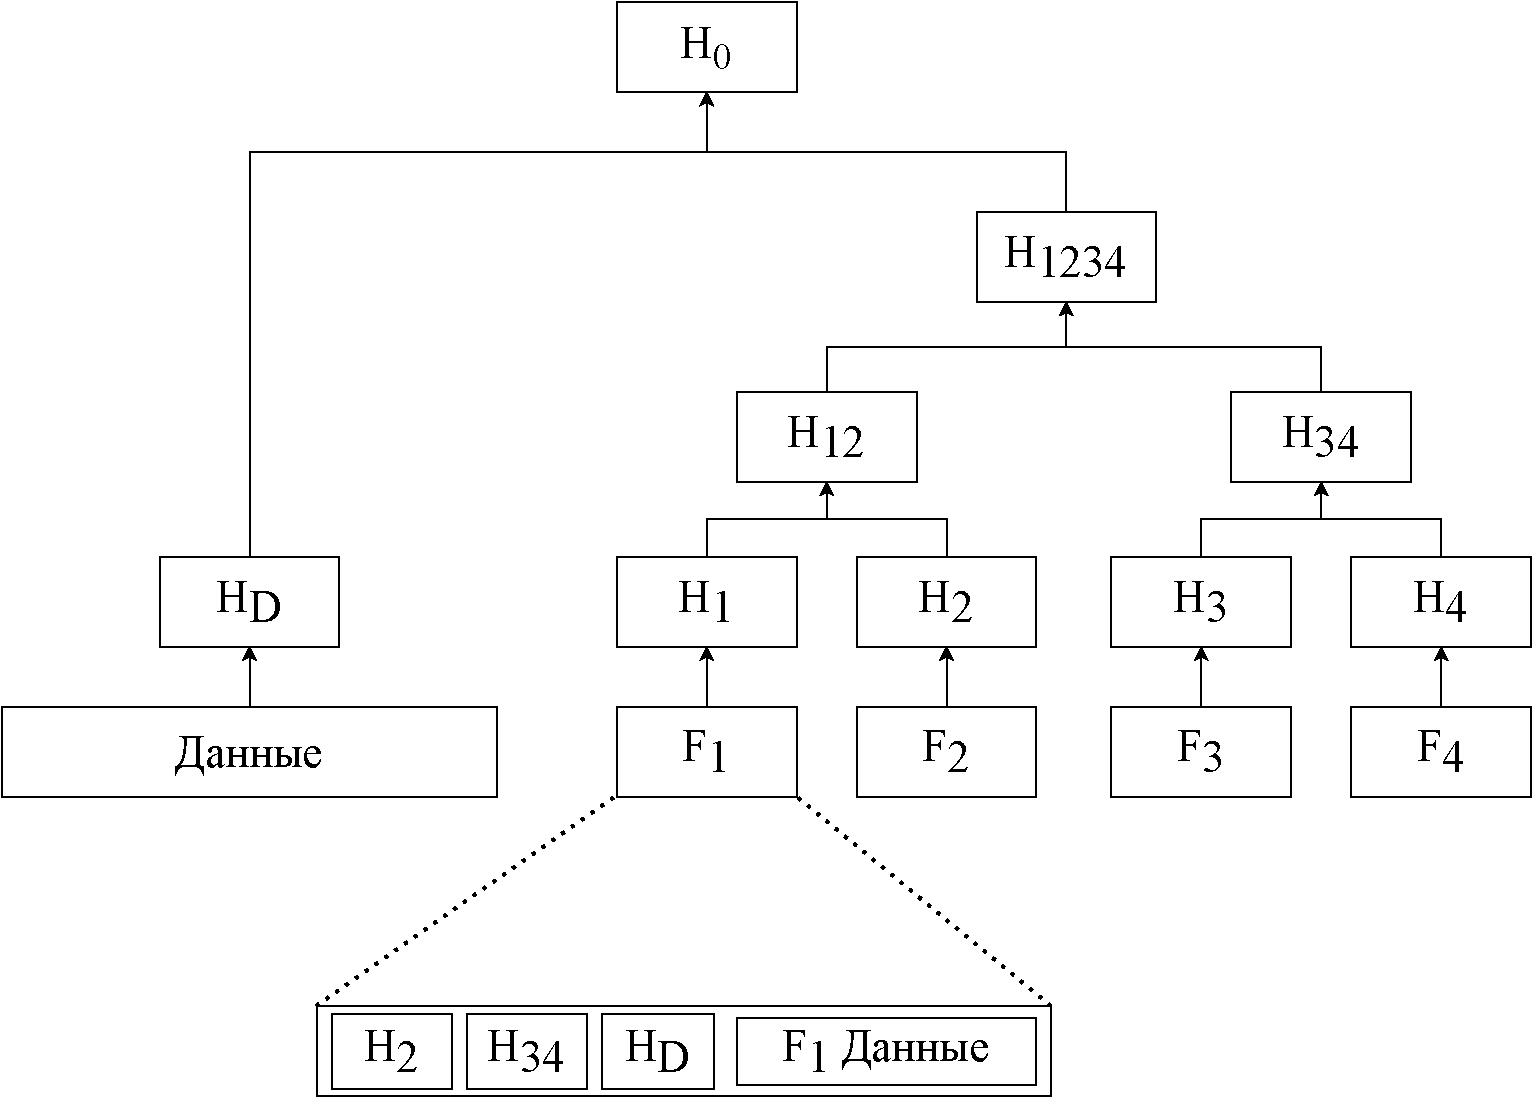
\includegraphics[width=\textwidth]{img/ocean.pdf}
	\caption{Пример дерева Меркла и фрагментов для OceanStore.}
	\label{fig:ocean}
\end{figure}

Данная система считается read-only, потому что изменение данных без изменения идентификатора невозможно, так как идентификатор создается на базе содержимого. Таким образом, например, при обновления версии каких-то данных, старая версия остается неизменной, но появляется новая версия с новым содержимым и GUID.

Данное хранилище, несмотря на внутренее устройство, поддерживает возможность иерархической структуры данных. Для этого требуется в некоторых объектах, которые не являются листьями дерева иерархии данных, хранить хеши дочерних вершин. GUID корня иерархической структуры известен.

На примере иерархической структуры видна сложность изменения данных: изменение элемента дерева приводит к необходимости изменения (замены на новый элемент) всех вершин-предков.

Как и хранилище из раздела \ref{par:pasis}, данная система защищена от частичного удаления или изменения данных, обладает возможностью восстановления, а также обладает возможностью доказательства изменения данных.

\subsubsection{Git}

Git \cite{git} --- система контроля версий. Данная система не решает задачу защиты от неправомерного доступа непосредественно, однако делает это косвенно: при нарушении целостности данных система перестанет работать, что будет являться доказательством неправомерного доступа. Внутреннее представление Git --- хранилище, адресующее по содержанию. Это означает, что файлы, которыми оперирует Git в рамках системной файловой системы, хранятся в виде ассоциативного массива, доступ в котором осуществляется по ключу. Данная система называется Object Store. В качестве ключа файла выступает хеш от его содержимого, подобно GUID в \ref{par:ocean}.

Иерархическую структуру файлов Git поддерживает в виде ориентированного ациклического графа Меркла за счет наличия 3 основных типов объектов:
\begin{enumerate}
	\item blob --- содержит информацию о конкретной версии файла. В ациклическом графе Меркла файлы этого типа всегда обладают нулевой степенью полуисхода, то есть их хеш составлен на основе содержимого файла. Этим же хешем данные файлы адресуются в упомянутом выше ассоциативном массиве.
	\item tree --- содержит информацию о конкретной версии директории. Данный объект содержит в себе другие объекты (больше 0), которые могут быть типа blob или tree. Он обладает отличной от обычной функцией суммирования: вместо простой конкатенации хешей вершин, в которые ведут дуги, в функции суммирования также фигурируют имена файлов дочерних вершин (реальные имена, не хеши), а также режимы доступа к данным файлам.
	\item commit --- содержит информацию о коммите --- фиксированном состоянии системы. commit обладает единичной степенью полуисхода и единственная его дуга ведет в объект типа tree, соотвествующей корневой директории репозитория. Объект типа commit хранит информацию об авторе изменений, связанных с коммитом, об имени, хеше и режиме доступа корневой директории и информацию о хеше родительского коммита --- то есть предыдущей зафиксированной версии. Адресуется коммит значением хеш функции от его содержимого. Схема, по которой описанный коммит связан с предыдущим, в точности соответствует схеме работы блокчейна.
\end{enumerate}

На рисунке \ref{fig:git1} схематично представлен пример графа для 3 основных типов объектов.

\begin{figure}[hbtp]
	\centering
	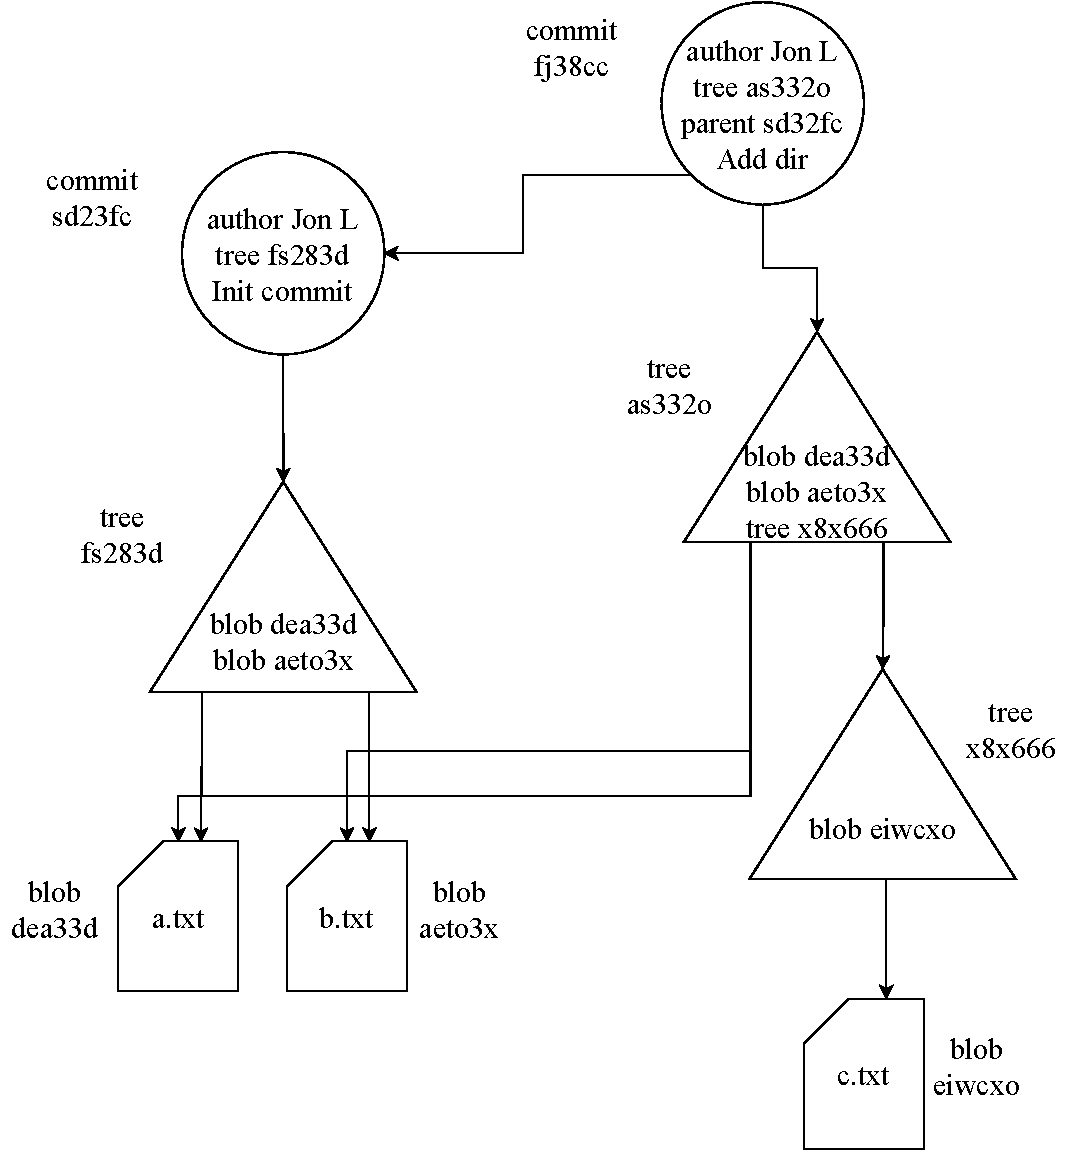
\includegraphics[width=\textwidth]{./img/git-mdag.pdf}
	\caption{Пример графа Меркла для 3 основных типов объектов}
	\label{fig:git1}
\end{figure}

Изменение внутренней структуры в процессе изменения данных происходит в 3 этапа:
\begin{enumerate}
	\item Изначально Git не будет учитывать изменения в рабочей директории, то есть при изменении файла у системы будет иметься копия файла из рабочей директории, которая не будет изменена.
	\item Чтобы система учла изменения, требуется добавить измененные файлы в индекс. Данное действие приведет к изменению файла с точки зрения файловой системы, с точки зрения внутреннего состояния системы Git это приведет к созданию нового объекта типа blob в Object Store, а также виртуального объекта типа tree (данный объект не будет виден в Object Store на этом этапе). Возможное состояние системы на этом этапе изображено на рисунке \ref{fig:git2}.
	\item При фиксации изменений виртуальный объект типа tree, соответствующий корню рабочей директории для новых версий файлов, добавленных в индекс, становится реальным, то есть создается объект в Object Store, а также создается объект типа commit, который ссылается (содержит хеш в качестве значения) на вновь созданный объект типа tree. Возможное состояние после всех проделанных действий изображено на рисунке \ref{fig:git3}.
\end{enumerate}

\begin{figure}[hbtp]
	\centering
	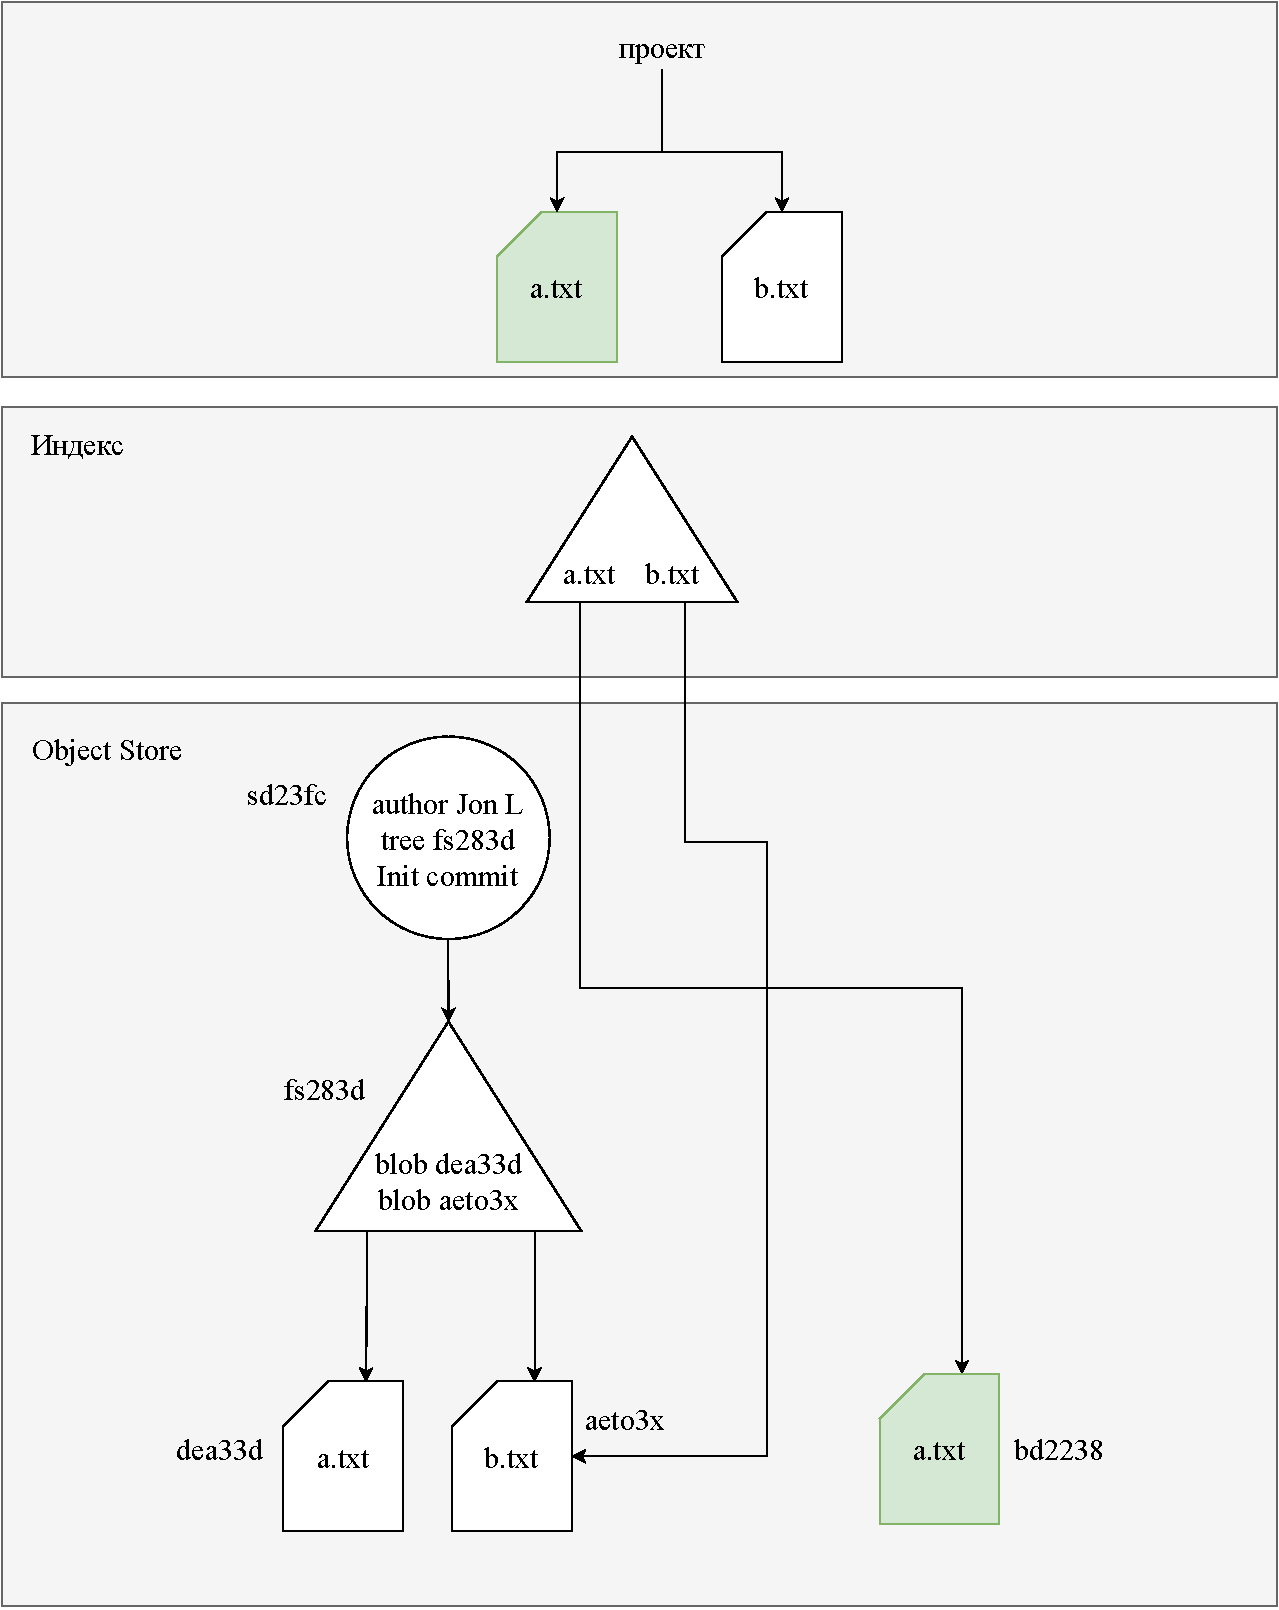
\includegraphics[width=\textwidth]{./img/git-add.pdf}
	\caption{Возможное состояние системы контроля версий Git при добавлении нового файла в индекс.}
	\label{fig:git2}
\end{figure}

\begin{figure}[hbtp]
	\centering
	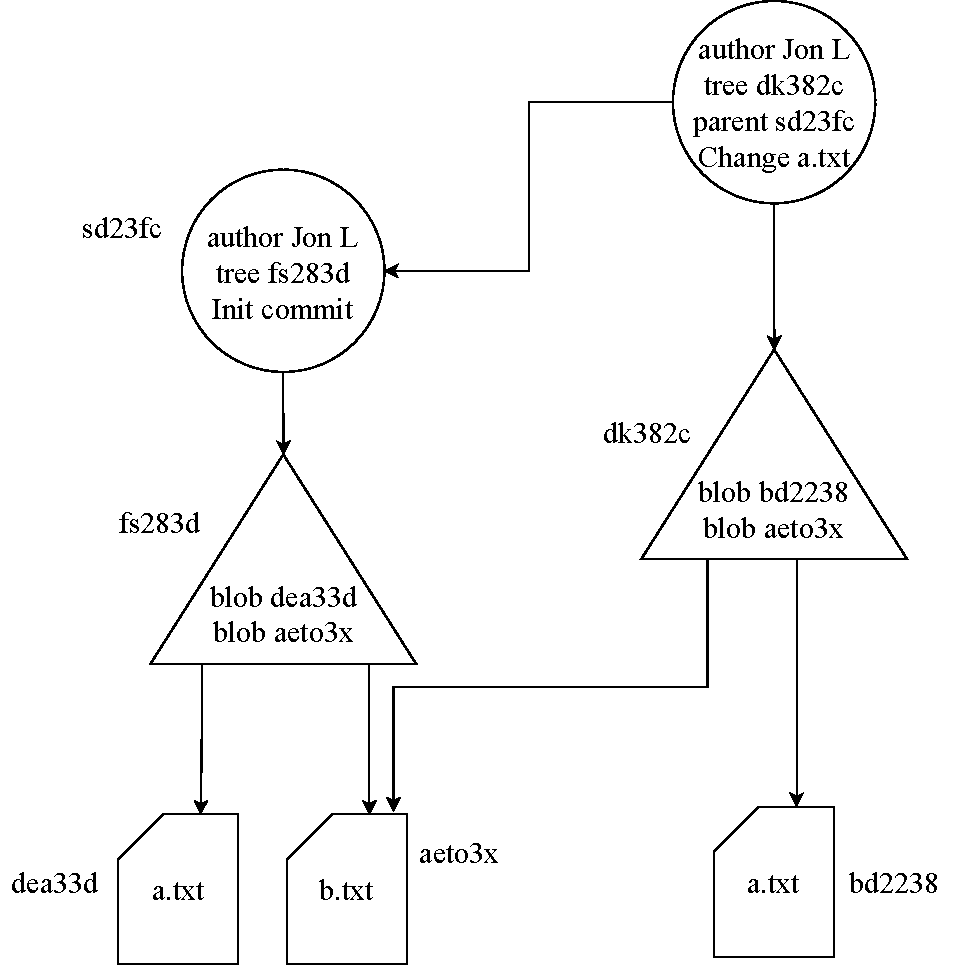
\includegraphics[width=\textwidth]{./img/git-commit.pdf}
	\caption{Возможное состояние системы контроля версий Git после фиксирования изменений.}
	\label{fig:git3}
\end{figure}

Неправомерный доступ подразумевает возможность доступа на запись к внутренней структуре, изменения в которой происходят исключительно за счет добавления новых объектов.

Возможны 3 варианта:
\begin{enumerate}
	\item Изменение содержимого объекта. Имя файла в системе Git --- его хеш и любое изменение содержимого приведет к несовпадению рассчитываемого хеша и имени файла, что приведет к ошибке и обнаружению нарушения в данных.
	\item Удаление объекта. Такая атака будет обнаружена в момент, когда произойдет попытка обращения к удаленному файлу. Он не будет найден в Object Store и будет ошибка.
	\item Добавление объекта. Добавление объекта не будет обнаружено, однако и данные, добавленные с новым объектом, не будут использованы ввиду того, что никакой другой объект не будет ссылаться на вновь созданный. Если добавить коммит в конце цепочки, то появляется возможность посчитать хеш вместе с хешем предыдущего commit объекта, однако подобный формат работы похож на стандартный и может быть осуществлен извне.
\end{enumerate}

Таким образом данная система обладает возможностью доказательства неправомерного изменения, а также удаления. Однако в общем случае возможно пересчитать значения хешей, на которые влияет изменение или удаление, что приведет к потере возможности доказательства.

\subsubsection{Bitcoin}

\label{par:bitcoin}

Bitcoin \cite{bitcoin} --- одноранговая децентрализованная электронная денежная система.

Для данной системы недопустимы сценарии, при которых данные теряются и приводится только доказательство неправомерного доступа к данным. Ввиду того, что данная система является распределенной, у нее нет единого хранилища данных, что усложняет получение неправомерного доступа к данным и их изменение или повреждение без возможности восстановления.

Транзакция --- операция передачи биткойнов с одного адреса на другой. Транзакция осуществляется следующим образом:

\begin{enumerate}
	\item Владелец биткойн-адреса (который связан с публичным ключом) использует любую совершенную транзакцию, в которой адресом назначения является данный адрес.
	\item Создается новая транзакция, которая содержит информацию о наборе адресов и соответсвующем количестве биткоинов, которые требуется перевести в рамках транзакции.
	\item Данная транзакция подписывается приватным ключом владельца кошелька, с которого происходит передача биткоинов.
\end{enumerate}

Таким образом невозможность неправомерного изменения транзакции обеспечивается за счет PKI \cite{pki}.

Транзакция является составным элементом блока. Блок --- составленный по определенным правилам набор транзакций.

Блок имеет определенную структуру, в которую входят:
\begin{itemize}
	\item[---] магическое число;
	\item[---] размер блока;
	\item[---] заголовок блока;
	\item[---] счетчик транзакций;
	\item[---] набор транзакций.
\end{itemize}

Заголовок блока состоит из следующих полей:
\begin{itemize}
	\item[---] версия блока;
	\item[---] хеш заголовка предыдущего блока;
	\item[---] хеш корня дерева Меркла, составленного из транзакций, входящих в данный блок;
	\item[---] текущее время;
	\item[---] целевое значение хеша, ниже которого должен быть хеш от заголовка;
	\item[---] число \textit{Nonce}, которое подбирается таким образом, чтобы хеш от заголовка был меньше целевого значения.
\end{itemize}

Блоки образуют блокчейн --- в заголовке очередного блока содержится хеш предыдущего блока, с помощью которого блоки собираются в цепь. Из одного блока может исходить несколько других блоков, которые содержат первый, как предшествующий. Действующей цепочкой считается наиболее длинная. В этом смысл концепции, называемой proof-of-work: большинство пользователей берут наиболее длинную цепочку блоков и коллективно пытаются подобрать требуемое значение \textit{Nonce}, которое бы удовлетворяло условию целевого значения, тем самым концентруя вычислительные мощности и не давая другим цепочкам стать длиннее текущей. Наиболее быстро будет рассчитываться та цепочка, для расчета которой используется наибольшее количество мощностей.

На рисунке \ref{fig:bitcoin} показана упрощенная схема хранения данных в системе Bitcoin.

\begin{figure}[hbtp]
	\centering
	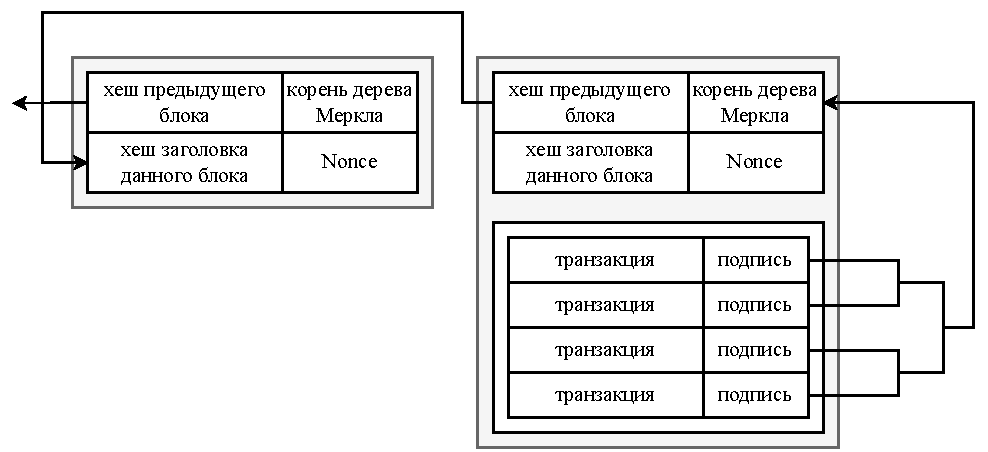
\includegraphics[width=\textwidth]{./img/bitcoin.pdf}
	\caption{Схема хранения данных в системе Bitcoin.}
	\label{fig:bitcoin}
\end{figure}

Сложность расчета значений \textit{Nonce} контролируется за счет изменения целевого значения хеша. Можно дать вероятностную оценку сложности вычисления нужного значения хеша в количестве попыток, исходя из следующих условий:
\begin{itemize}
	\item[---] значение хеш функции является случайным значением;
	\item[---] число ведущих нулей в бинарном представлении целевого значения равняется числу $M$.
\end{itemize}

Тогда вероятность появления такого значения хеша, которое будет меньше целевого значения, равна вероятности выпадения $M$ первых нулей при расчете хеша и рассчитывается по формуле \ref{eq:pnce}.

\begin{equation}
\label{eq:pnce}
P = \frac{1}{2^M},
\end{equation}

С учетом независимости расчетов для различных $Nonce$ и формулы \ref{eq:pnce}, можно рассчитать количество попыток, требуемых совершить в среднем для получения одного удовлетворяющего числа по формуле \ref{eq:enonce}.

\begin{equation}
\label{eq:enonce}
N = \frac{1}{\frac{1}{2^M}} = 2^M,
\end{equation}

Наиболее известный способ атаки на системы, работающие по концепции proof-of-work --- атака 51\%. Суть атаки заключается в том, что атакующий владеет большинством вычислительных мощностей и делает следующие действия:
\begin{enumerate}
	\item Сделать блок, который будет содержать некоторую транзакцию $T_1$.
	\item Дождаться, пока система, на счет которой мы перевели биткоины, будет считать транзакцию $T_1$ завершившейся.
	\item Взять блок, предшествующий блоку из пункта 1, и начать делать новую цепочку без транзакции $T_1$ до тех пор, пока она не станет действующей.
\end{enumerate}

Такая атака позволяет неправомерно изменить данные.

\pagebreak

\subsubsection*{Выводы}


Сравнение рассмотренных методов хранения данных с возможностью защиты от неправомерного доступа можно увидеть в таблице \ref{tab:res}. Обозначения:
\begin{itemize}
    \item[---] НД --- неправомерное действие;
    \item[---] КФС --- криптографические файловые системы;
    \item[---] У --- удаление блока;
    \item[---] И --- изменение;
    \item[---] ЧУ --- частичное удаление блока;
    \item[---] ЧИ --- частичное изменение.
\end{itemize}

Полученные результаты можно свести к следующему:
\begin{itemize}
    \item[---] Защита от чтения возможна в системе, в которой определенная группа людей обладает некоторым уникальным знанием (ключ в КФС).
    \item[---] Восстановление данных после частичного изменения или удаления блока возможно в распределенных системах, использующих стирающий код, в связи с тем, что фрагменты хранятся в разных местах и допускается неправомерный доступ в части мест.
    \item[---] Исключает возможность полного неправомерного изменения только Bitcoin, потому что во всех рассмотренных системах количество узлов, в которых хранятся данные, конечно и задано наперед (хоть и в теории может быть очень велико), в то время как в Bitcoin все узлы системы содержат одно состояние.
    \item[---] Возможностью доказательства неправомерного изменения обладают все системы кроме КФС, используя для этого контрольные суммы и хеши. Однако также как в случае удаления, в локальной системе без шифрования нарушитель может восстановить целостность цепочки блоков при изменении внутреннего состояния Git.
    \item[---] Возможностью доказательства неправомерного удаления блока обладают 2 системы, в основе которых лежит блокчейн. Однако если данные не шифруются никаким образом, то в случае с Git человек, нарушающий права, способен повторить действия самой системы, и произвести изменения, поддержав целостность цепочки блоков.
\end{itemize}

\begin{table}[h]
    \begin{center}
        \caption{Методы хранения и обеспечиваемая защита.}
        \label{tab:res}
        \begin{tabular}{|c|c|c|c|c|c|}
            \hline
            \bfseries НД & \bfseries PASIS & \bfseries КФС & \bfseries OceanStore & \bfseries Git & \bfseries Bitcoin  \\
            \hline
            чтение (исключение) & - & + & - & - & - \\ \hline
            ЧУ или ЧИ (восстановление) & + & - & + & - & - \\ \hline
            У или И (исключение) & - & - & - & - & + \\ \hline
            изменение (доказательство) & + & - & + & +/- & + \\ \hline
            удаление (доказательство) & - & - & - & +/- & + \\ \hline
        \end{tabular}
    \end{center}
\end{table}

\clearpage

\subsection{Метод хранения данных в СУБД ClickHouse}

ClickHouse --- колоночная СУБД \cite{ch}. Блоки данных, которые хранит СУБД, физически поделены на столбцы, а не на строки. Формат хранения данных не единый и зависит от используемого движка, движок задается для каждой таблицы. Разные движки имеют один и тот же интерфейс, оперируют общими структурами, однако внутреннее строение отличается. В рамках данной работы рассматривается движок MergeTree \cite{mergetree}.

\subsubsection{Движок MergeTree}

Звено --- блок, в виде которого движок хранит данные \cite{mergetreearch}. Физически определяется как директория на диске, хранящая в себе файлы, с информацией о данных, индексах, хеш-суммах и другой метаинформацией.

Партиция --- логическая группа звеньев, определяемая по заранее известному признаку \cite{mergetreearch}. Таким признаком, например, может быть неделя, к которой принадлежат данные. Физически определяется как составная часть имени звена, каждое звено принадлежит только 1 партиции. Например, если недели идентифицируются датой понедельника, то название звена хранит в себе дату понедельника недели, в которую он (и все данные, входящие в него) входит. Партиции образуют непересекающиеся группы данных, что позволяет эффективнее выполнять операцию поиска.

Операция слияния звеньев --- объединение подмножества звеньев в 1 звено, содержащий все данные объединяемого подмножества \cite{mergetreearch}. Данный подход используется для исключения большого количества перезаписи данных для сохранения требуемого порядка элементов. Из того, что звено принадлежит только 1 партиции, следует, что объединение блоков, принадлежащих разным партициям не происходит.

Идея движка MergeTree заключается в том, что приходящие блоки с данными разбиваются на звенья по признаку партиции, полученные звенья отсортированы по первичному ключу, записываются в БД, а затем над некоторыми подмножествами звенья в асинхронном режиме выполняется операция слияния для более эффективного хранения и поиска.

Каждое звено данных логически делится на гранулы. Гранула --- минимальный набор данных (множество элементов), который считывается движком при выборке данных \cite{mergetreearch}. Гранула также является единицей индексации данных: индексируются только первые элементы каждой гранулы. Для каждого звена данных движок создает файл с засечками (индексный файл). Для каждого столбца, независимо от того, входит он в первичный ключ или нет, сохраняются эти же засечки. Засечки используются для поиска данных напрямую в файлах столбцов. Размер гранул оганичен настройками движка по количеству и байтам. Количество строк в грануле лежит в диапазоне не больше максимально заданного значения, в зависимости от размера строк. Размер гранулы может превышать максимально заданный размер в байтах в том случае, когда размер единственной строки в грануле превышает значение настройки. В этом случае, размер гранулы равен размеру строки.

Описанные выше концепции показаны на рисунке \ref{fig:clickhousebase}.

\begin{figure}[hbtp]
	\centering
	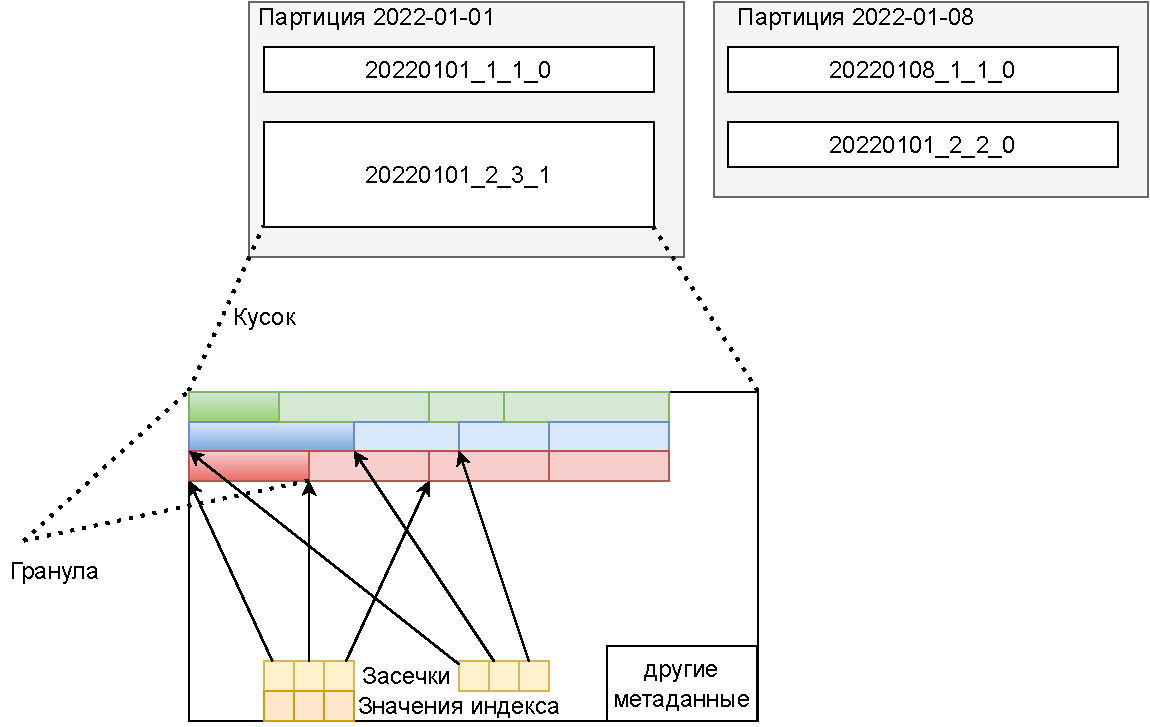
\includegraphics[width=\textwidth]{img/clickhousebase.pdf}
	\caption{Структура хранения данных в СУБД ClickHouse.}
	\label{fig:clickhousebase}
\end{figure}

\subsubsection{Хранение данных в файловой системе}

Существует 2 вида физического хранения столбцов звена в MergeTree:
\begin{itemize}
    \item [---] компактный \cite{datapartcompact};
    \item [---] широкий \cite{datapartwide}.
\end{itemize}

Отличие заключается в том, что компактный вид хранит все столбцы в 1 файле, а широкий --- в разных. Примеры компактного и широкого хранения столбцов звена показаны на рисунках \ref{fig:compactstore} и \ref{fig:widestore}. Для всех файлов в движке считается хеш-сумма, для файлов с данными считаются 2 --- для данных в сжатом виде и в расжатом. Поэтому при компактном хранении для данных будет 1 хеш-сумма, а при широком будет соответствовать количеству столбцов.

\begin{figure}[hbtp]
	\centering
	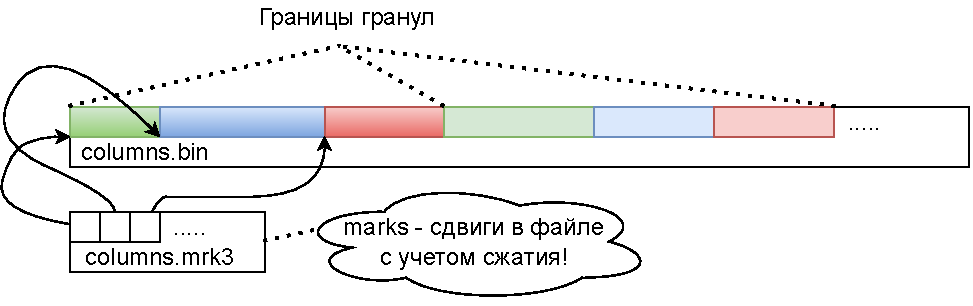
\includegraphics[width=\textwidth]{img/compactstore.pdf}
	\caption{Компактное хранение столбцов.}
	\label{fig:compactstore}
\end{figure}

\begin{figure}[hbtp]
	\centering
	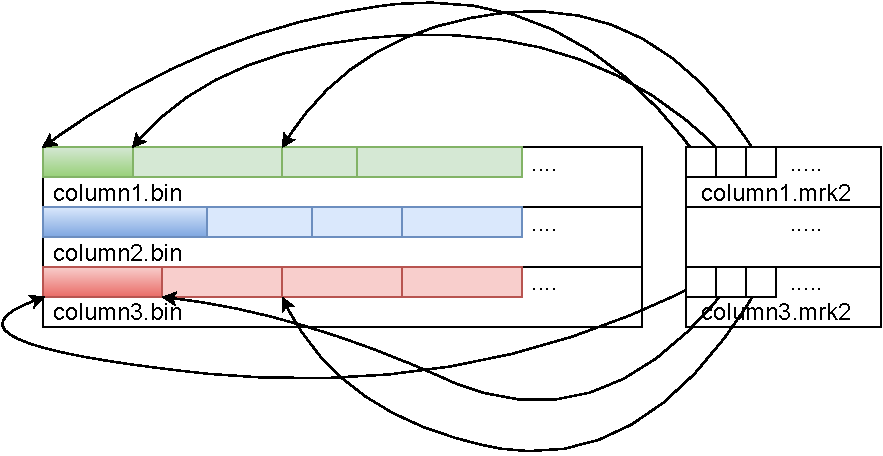
\includegraphics[width=\textwidth]{img/widestore.pdf}
	\caption{Широкое хранение столбцов.}
	\label{fig:widestore}
\end{figure}

Для записи данных используется класс \texttt{WriteBuffer}. При обоих видах хранения данные пишутся через 4 буфера (в скобках указаны соответствующие имена переменных):
\begin{itemize}
    \item [---] хеш-буфер (\texttt{hashing\_buf}) \cite{hashingbuf} --- считает хеш-сумму несжатых данных;
    \item [---] сжимающий буфер (\texttt{compressed\_buf}) \cite{compressingbuf} --- сжимает данные;
    \item [---] хеш-буфер (\texttt{plain\_hashing}) \cite{hashingbuf} --- считает хеш-сумму сжатых данных;
    \item [---] файловый буфер (\texttt{plain\_file}) \cite{filebuf} --- буферизует данные для более эффективной записи в файл.
\end{itemize}

В действительности данные буферизуются только на 2 уровнях: на уровне сжимающего и файлового буферов. Хеш-буферы при поступлении очередных данных используют поток байт для расчета хеш-суммы и сразу же перенаправляют в нижележащие буферы. Сжимающий буфер, помимо сжатия, считает хеш-сумму для каждого сжатого блока данных. Схема показана на рисунке \ref{fig:bufscheme}. Размер буферов по умолчанию --- 1 Мб. Буфер сбрасывается при достижении 1 из 2 условий:
\begin{itemize}
	\item [---] буфер переполнился;
	\item [---] записался целиком столбец гранулы (даже при компактном хранении, для более оптимального чтения).
\end{itemize}

\begin{figure}[hbtp]
	\centering
	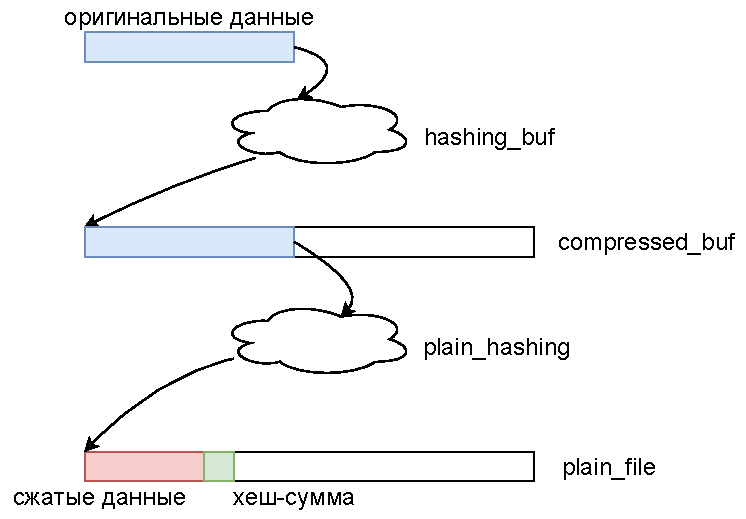
\includegraphics[width=\textwidth]{img/bufscheme.pdf}
	\caption{Схема записи с 4 буферами.}
	\label{fig:bufscheme}
\end{figure}

\subsubsection{Вставка данных}

Вставка звена данных происходит в 2 шага:
\begin{itemize}
	\item [---] создается временное звено, данные пишутся в него \cite{inserttemp};
	\item [---] если данные успешно записываются, то временное звено переименовывается в обычное \cite{insertrename}.
\end{itemize}

Такая схема решает проблему, связанную с битыми звеньями: если вставка не проходит, то звено остается временным и удаляется.

\subsubsection{Слияния и мутации звеньев}

Слияния звеньев, как и мутации, происходят в фоновом режиме и состоят из следующих этапов \cite{backgroundproc}:
\begin{itemize}
	\item [---] запуск планировщика фоновых задач;
	\item [---] выбор звеньев, которые можно слить или мутировать;
	\item [---] постановка задачи обработки выбранных звеньев в очередь на выполнение фоновому пулу потоков.
\end{itemize}

Сами задачи выполняются пошагово. Каждая задача имеет метод \texttt{bool execute()}, который возвращает \texttt{false}, когда задача выполнена, и \texttt{true} в обратном случае. Класс, выполняющий задачу, вызывает данный метод до тех пор, пока задача не будет выполнена. Такое дробление задачи на части позволяет откладывать фоновые задачи при повышенной нагрузке системы, лучше планировать, снижая приоритет долгим задачам.

И в случае с мутациями, и в случае со слияниями результатом задачи всегда является один звено. Задача сохранения целостности решается похожим на вставку образом: все операции происходят со временным звеном, а последним шагом является переименование в обычный. Однако в отличие от вставок, данные операции содержат звенья, которые становятся неактуальными и которые нужно убрать. Данная задача в слияниях и мутациях решается по-разному.

Имена звеньев создаются по шаблону и состоят из следующих частей \cite{datapart}:
\begin{itemize}
	\item [---] имя партиции, к которой принадлежит звено;
	\item [---] минимальный номер вставленного звена, который был слит в текущий;
	\item [---] максимальный номер вставленного звена, который был слит в текущий;
	\item [---] версия звена с точки зрения слияний (инкрементируется каждый раз, когда происходит слияние);
	\item [---] версия звена c точки зрения мутаций (разделяет номер со вставляемыми звеньями для возможности определения необходимости применения мутации к отдельным звеньям).
\end{itemize}

В слияниях неактуальные звенья узнаются из версии. Пусть имеется 3 звена: \texttt{all\_1\_1\_0},  \texttt{all\_2\_2\_0}, \texttt{all\_3\_3\_0}. При слиянии новое звено получит имя: \texttt{all\_1\_3\_1}. Старые 3 звена будут покрыты \cite{covered} новым и будут удалены при завершении работы сервера или при перезапуске.

В мутациях неактуальные звенья также узнаются из версии, но из другой. Более того, мутации происходят поочередно над каждым звеном (несколько звеньев не могут участвовать в мутации), при этом к одному звену может применяться несколько мутаций одновременно.

Покрывающие звенья в операциях слияния и мутаций показаны на рисунке \ref{fig:cover} зеленым цветом, покрываемые --- красным.

\begin{figure}[hbtp]
	\centering
	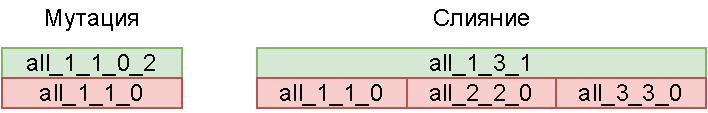
\includegraphics[width=\textwidth]{img/cover.pdf}
	\caption{Покрывание старых звеньев новыми при мутациях и слияниях.}
	\label{fig:cover}
\end{figure}

Такой алгоритм действий позволяет избежать неконсистентного состояния: атомарно выполняется 1 операция (переименования звена), остальные операции выполняются как следствие покрытия.

\subsubsection{Шифрование данных}

В ClickHouse доступно шифрование на уровне диска, указанного в конфигурационном файле. Реализовано оно схожим со сжатием образом: поверх буфера записи в файл находится буфер шифрования. Алгоритм шифрования --- AES с ключами размеров 128, 192, 256 бит. В отчете NIST \cite{nist} за 2019 год указано, что AES допустимо использовать как алгоритм блочного шифрования до 2030 года с любой из перечисленных длиной ключа.

Также доступно шифрование столбцов тем же алгоритмом, которое реализовано в виде кодека. Допустимо использования нескольких кодеков одновременно, что позволяет сжимать и шифровать данные одновременно.

\subsubsection{Проверка целостности данных}

Проверка целостности для каждого звена состоит из следующих шагов:
\begin{itemize}
	\item [---] проверить вычисленные значения хеш-сумм всех сжатых блоков с записанными значениями;
	\item [---] проверить вычисленное значение хеш-суммы для сжатых данных из файла с данными (или файлов при широком хранении) с записанным значением;
	\item [---] проверить вычисленное значение хеш-суммы для расжатых данных файла с данными (или файлов при широком хранении) с записанным значением;
	\item [---] проверить вычисленные значения хеш-сумм для файлов с метаданными с записанными значениями.
\end{itemize}

Все метаданные, помимо файловой системы, кэшируются в оперативной памяти, в том числе информация об активных звеньях и хеш-суммах. При изменении данных поменять закэшированное в оперативной памяти значение хеш-суммы не получится, однако при перезагрузке СУБД значения можно подменить так, что бы было невозможно доказать изменение или удаление данных.

В случае изменения данных придется пересчитать 3 хеш-суммы (у сжатого блока, у сжатого файла и у расжатых данных), а в случае удаления звена состояние будет оставаться валидным без дополнительных действий.

\subsubsection{Анализ защиты от неправомерного доступа в движке MergeTree}

С учетом выводов \ref{par:mainanal} и того, что движок MergeTree не является распределенным, можно сделать следующие выводы:
\begin{enumerate}
	\item При отсутствии шифрования, злоумышленник обладает возможностью делать действия, аналогичные действиям лица, обладающего нужным доступом к информации, в связи с чем система не имеет никакой защиты.
	\item При наличии шифрования:
	\begin{itemize}
		\item [---] исключается возможность неправомерного чтения;
		\item [---] есть возможность доказательства неправомерного изменения.
	\end{itemize}
\end{enumerate}

Возможность доказательства неправомерного удаления целого звена отсутствует.

\subsection{Добавление возможности доказательства неправомерного удаления в MergeTree}

Для обеспечения возможности доказательства неправомерного удаления можно сделать:
\begin{enumerate}
	\item расчет хеш-суммы на основе информации обо всех звеньях;
	\item расчет хеш-сумм звеньев зависимым от метаданных (хеш-сумм) других звеньев.
\end{enumerate}

Данные подходы решают задачу по-разному: в первом случае мы будем иметь одно значение, во втором --- количество значений будет совпадать с количеством звеньев. Первый подход меньше взаимодействует с файловой системой, в следствие чего быстрее работает, второй подход дает возможность определить, на каком элементе нарушается консистентность (при условии, что данные не будут меняться после нарушения консистентности).

Пусть $y_i$ --- искомые хеш-суммы. Пусть для определенности новые хеш-суммы (относящиеся не к конкретному звену, а поддерживающие некоторые связи) будут называться \textit{цепью хеш-сумм} в случае со множеством хеш-сумм, и \textit{результатом цепи хеш-сумм} в случае хранения 1 значения.

\pagebreak

Тогда единственная хеш-сумма на основе информации обо всех звеньях может рассчитываться по формуле \ref{eq:concat}, подобно тому, как это делается в \ref{par:pasis}, либо по формуле \ref{eq:hashchain} подобно тому, как это делается в \ref{par:bitcoin}.
\begin{equation}
\label{eq:concat}
y_0 = hash(x_1 | x_2 | ... | x_n),
\end{equation}

\begin{equation}
\label{eq:hashchain}
y_0 = hash(x_n | hash(x_{n-1} | ...)),
\end{equation}

где $hash$ --- хеш-функция, $n$ --- количество звеньев данных, $|$ --- операция конкатенации строк, $x_i$ --- метаданные $i$-ого звена.

Хеш-суммы звеньев, зависимых от метаданных других звеньев, могут вычисляться по рекуррентной формуле \ref{eq:rec}, похожей на \ref{eq:hashchain}, но с запоминанием промежуточных состояний.

\begin{equation}
\label{eq:rec}
y_i = hash(x_i|y_{i-1}), y_1 = hash(x_1).
\end{equation}

В рамках данной работы будет использоваться подход с хранением 1 значения для цепи хеш-сумм ввиду того, что при первом нарушении консистентности и происхождении новых событиях информация о месте нарушения связи может стать невалидной и давать неверную информацию.

\subsubsection{Атомарные операции для избежания неконсистентного состояния}

Операции изменения состава активных партов и пересчета хеш-сумм --- сильно связанные операции. Если выполнится одна операция, но не выполнится другая, то состояние будет несогласованным. В связи с чем данные операции должны выполняться атомарно: либо обе выполниться, либо обе не выполниться. В СУБД атомарность \cite{atomicity} --- одно из требований, предъявляемых к транзакциям. Одно из решений, позволяющих удовлетворить требованию атомарности --- журналирование \cite{journaldbms}. Перед началом выполнения операций, данные операции записываются в журнал, и только после этого начинают выполняться. В случае сбоев, состояние БД сверяется с операциями, записанными в журнале, после чего операции либо доделываются до конца транзакции, либо откатываются.

Таким образом атомарность операции будет обеспечиваться за счет следующей последовательности шагов:
\begin{enumerate}
	\item запись новых значений хеш-сумм в журнал;
	\item изменение состава активных звеньев с помощью переименовывания;
	\item запись новых значений хеш-сумм из журнала в файл.
\end{enumerate}

Данная схема допускает сбой на любом шаге:
\begin{enumerate}
	\item При сбое на 1 шаге, обе операции будут считаться невыполненными.
	\item При сбое на 2 шаге, обе операции все так же будут считаться невыполненными, значение из журнала не используется, потому что значение из файла будет соответствовать составу активных звеньев.
	\item При сбое на 3 шаге обе операции будут считаться выполненными: произойдет несовпадение хеш-суммы из файла и хеш-суммы активных звеньев, однако нужное значение хеш-суммы для файла будет получено из журнала и записано в файл.
\end{enumerate}

\subsection{Выводы}

В данном разделе были классифицированы неправомерные действия, методы защиты от них, были рассмотрены существующие решения в области хранения данных с защитой от неправомерного доступа, выделены основные элементы, позволяющие обеспечить определенные методы защиты. Также была рассмотрена СУБД ClickHouse, в частности движок MergeTree: была проанализирована структура хранения данных, порядок записи, слияния и изменения порций данных, называемых звеньями. Был проведен анализ защищенности от неправомерного доступа в движке MergeTree и предложено улучшение текущего метода хранения данных для обеспечения возможности доказательства неправомерного удаления данных.

\pagebreak